\documentclass[titlepage]{article}
\usepackage[margin=0.6in]{geometry}
\usepackage{graphicx}
\usepackage{wrapfig}
\usepackage{lscape}
\usepackage{rotating}
\usepackage{epstopdf}
\renewcommand{\baselinestretch}{1.5} 

\author{
	\textbf{Oyedotun Oyesanmi } 
	\and 
	\textbf{Ming-Zhen Ling}}
\title{Database Management System - Project\\Phase 1}
\begin{document}
\maketitle
\pagebreak
\begin{figure}[ht]
\centering
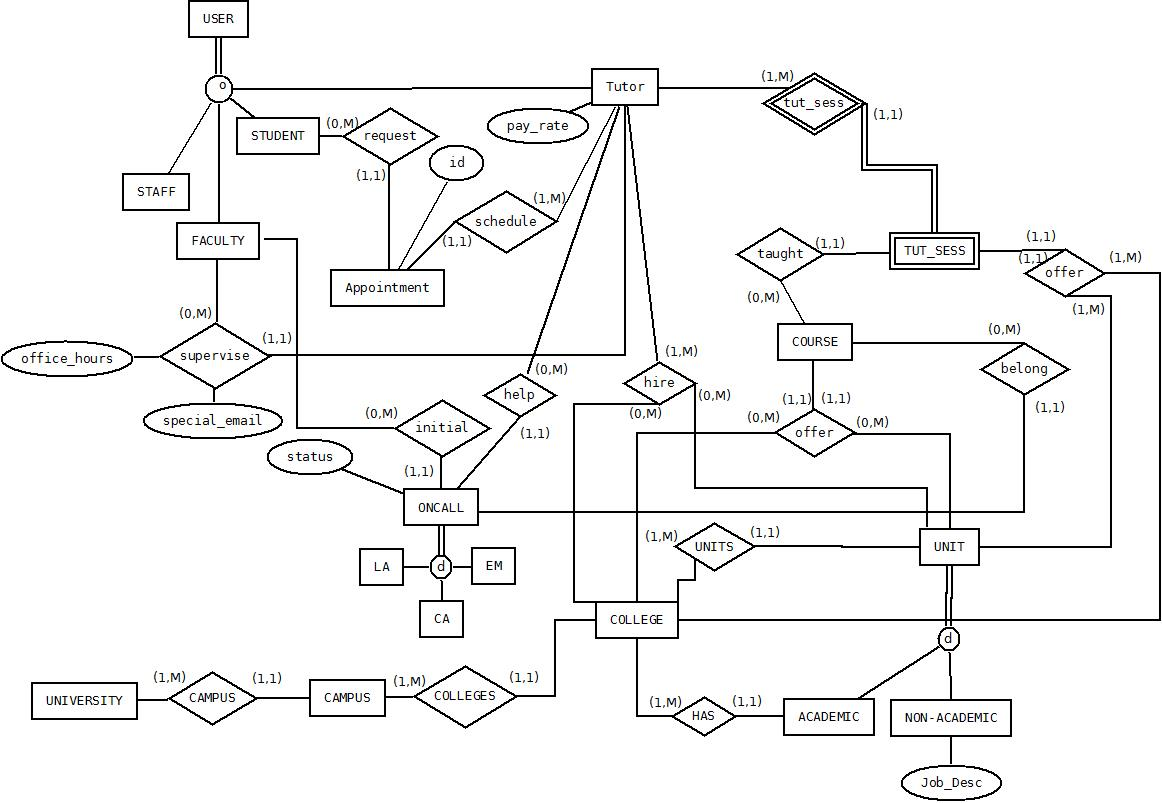
\includegraphics[trim=3cm 0cm 0cm 3cm, clip=false, totalheight=0.5\textheight, angle=90]{Relationship-Phase1.jpeg}
\clearpage
\end{figure}

\begin{figure}[ht]	
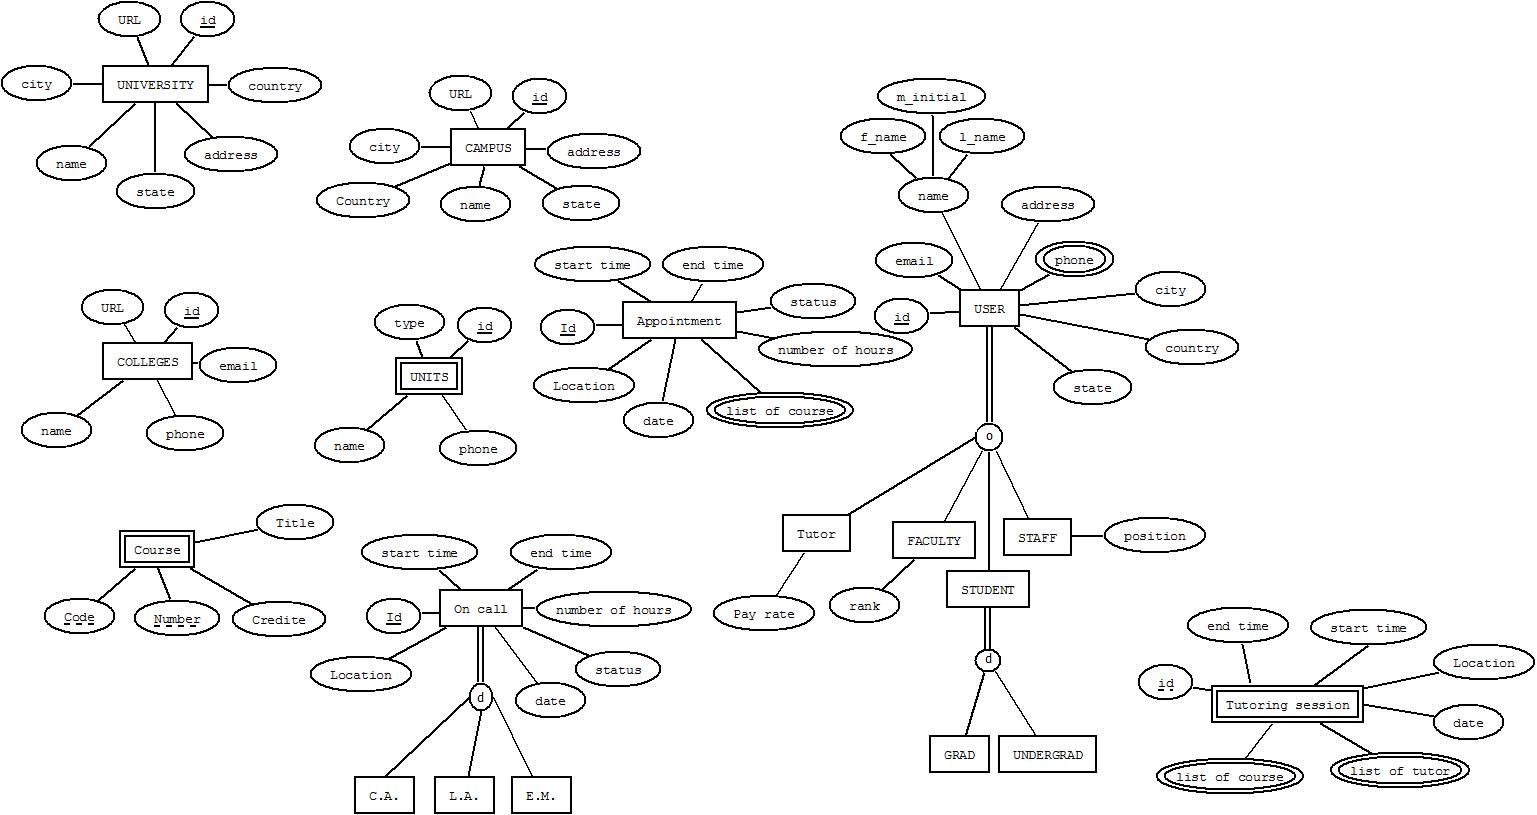
\includegraphics[trim=0cm 0cm 0cm -1cm, clip=false, totalheight=0.56\textheight, angle=90]{Entity-Phase1.jpeg} 
\end{figure}
\clearpage

\textbf{ASSUMPTIONS}
\begin{enumerate}
	
	\item A tutor must have an appointment.
	\item One faculty may or may not initiate an on call.
	\item One faculty can initiate many on calls.
	\item A tutor may or may not help an on call.
	\item A unit or college may or may not hire tutor.
	\item A tutor has to teach at least one course.
	\item A university must have at least one campuses.
	\item A campus must have at least one colleges.
	\item A colleges must have at least one unit.
	\item A unit or college must offer at least one tutoring session.
	\item A tutor must have at least one tutoring session.
	\item A course may or may not have tutoring session.\\\\
	
\end{enumerate}

\textbf{ABBREVIATIONS USED}
\begin{enumerate}
	
	\item L.A.  - Laboratory Assistant
	\item C.A. - Classroom Assistant
	\item E.M. - Exam Monitoring

\end{enumerate}
\end{document}